\documentclass[../../main.tex]{subfiles}
\begin{document}

{\bf [解]}
\paragraph{(1)}

与えられた関数
\begin{align}
  f(x) = \dfrac{x+t}{x(1-tx)} \label{eq:1}
\end{align}
について考える．
一階微分は
\begin{align}
  f'(x) = \dfrac{t(x^2 + 2tx - 1)}{x^2 (1-tx)^2} \label{eq:2}
\end{align}
だから$f(x)$の増減表は以下のようになる．
\begin{table}[htb]
  \centering
  \caption{$f(x)$ の増減表}
  \begin{tabular}{c|c|c|c|c|c}
    $x$ & $0$ & $\dots$ & $-t + \sqrt{t^2+1}$ & $\dots$ & $1$ \\ \hline
    $f'$ & & $-$ & $0$ & $+$ & \\ \hline
    $f$ & & $\searrow$ & & $\nearrow$ &
  \end{tabular}
\end{table}
従って$f(x)$の極小値を与える$x$は
\begin{align}
  \alpha = -t + \sqrt{t^2+1} \label{eq:3}
\end{align}
である．$t$が$0\le t \le 1$の範囲で動く時の$(\alpha,f(\alpha))$の挙動を調べよう．
$f(\alpha)$は\cref{eq:3}より
\begin{align}
  f(\alpha)
  &= \dfrac{\alpha+t}{\alpha(1-t\alpha)} \\
  &= \dfrac{\sqrt{1+t^2}}{\alpha(1+t^2-t\sqrt{t^2+1})} \\
  &= \dfrac{1}{\alpha(\sqrt{1+t^2}-t)} \\
  &= \dfrac{1}{\alpha^2} \label{eq:4}
\end{align}
である．$\alpha$を$t$で微分すると
\begin{align}
  \alpha' = \dfrac{-\alpha}{\sqrt{t^2+1}} \label{eq:5}
\end{align}
であることに注意して$f(\alpha)$を$t$で微分すると
\begin{align}
  \dfrac{d}{dt} f(\alpha)
  &= \dfrac{d\alpha}{dt}\dfrac{f(\alpha)}{d\alpha} \\
  &= \dfrac{-\alpha}{\sqrt{t^2+1}}\dfrac{1}{\alpha^2} \\
  &= \dfrac{-1}{\alpha\sqrt{t^2+1}}
\end{align}
である．\cref{eq:3}より$0<t<1$では$\alpha>0$だから，$\dfrac{d}{dt} f(\alpha)>0$である．
従って$f(\alpha)$の増減表は以下のようになる．

\begin{table}[htb]
  \centering
  \caption{$\alpha, f(\alpha)$ の $t$ に関する増減表}
  \begin{tabular}{c|c|c|c}
    $t$ & $0$ & $\dots$ & $1$ \\ \hline
    $d\alpha/dt$ & & $-$ & \\ \hline
    $df/dt$ & & $+$ & \\ \hline
    $(\alpha, f(\alpha))$ & $(1, 1)$ & $\nwarrow$ & $(\sqrt{2}-1, 3+2\sqrt{2})$
  \end{tabular}
\end{table}

よって，$t$を動かした時の$(\alpha,f(\alpha))$の軌跡は下図のようになる．ただし端点は除く．

\begin{figure}[htb]
  \centering
  \begin{tikzpicture}[xscale=1.5, yscale=0.9, >=stealth, every node/.style={font=\small}]

    % --- 1. 定数定義 ---
    % t = 1: alpha = sqrt(2) - 1 ≈ 0.4142, f(alpha) = 2 / (sqrt(2)-1) = 2(sqrt(2)+1) = 3 + 2*sqrt(2) ≈ 4.8284
    % (注: 2/(sqrt(2)-1) = 2(sqrt(2)+1) ≈ 4.828)
    % t -> 0: alpha -> 1, f(alpha) -> 2
    \def\xMin{0.41421} % sqrt(2) - 1
    \def\yMax{5.82842} % (sqrt(2) + 1)^2
    \def\xMax{1.0}
    \def\yMin{1.0}

    \coordinate (A) at (\xMax, \yMin);
    \coordinate (B) at (\xMin, \yMax);

    % --- 2. 座標軸 ---
    \draw[->, thick] (-0.08, 0) -- (1.2, 0) node[right] {$\alpha$};
    \draw[->, thick] (0, -0.4) -- (0, 7) node[above] {$f(\alpha)$};
    \node[below left=2pt] at (0, 0) {$O$};

    % --- 3. 補助線（点線） ---
    \draw[dashed, gray!70] (\xMax, 0) -- (A) -- (0, \yMin);
    \draw[dashed, gray!70] (\xMin, 0) -- (B) -- (0, \yMax);

    % --- 4. 厳密な軌跡曲線 Y = 2 / X の描画 ---
    \draw[very thick, blue!80!black, domain=\xMin:\xMax, samples=80]
    plot (\x, {1.0 / (\x)^2});

    % 進行方向矢印 (t が 0 -> 1 で alpha は 1 -> sqrt(2)-1 へ減少)
    \draw[->, very thick, blue!80!black]
    (0.72, {2.0 / 0.72}) -- (0.68, {2.0 / 0.68});
    % \node[blue!80!black, above right, font=\footnotesize] at (0.7, {2.0 / 0.7}) {$t$ 増加方向};

    % --- 5. 軸目盛りラベル ---
    \node[below=2pt] at (\xMax, 0) {$1$};
    \node[left=2pt]  at (0, \yMin) {$2$};
    \node[below=2pt] at (\xMin, 0) {$\sqrt{2}-1$};
    \node[left=2pt]  at (0, \yMax) {$2(\sqrt{2}+1)$};

    % --- 6. 端点（除外点のため白丸） ---
    \draw[thick, blue!80!black, fill=white] (A) circle (1.8pt);
    \draw[thick, blue!80!black, fill=white] (B) circle (1.8pt);

    % 軌跡ラベル
    \node[blue!80!black, font=\normalsize] at (0.85, 3.8) {$f(\alpha) = \dfrac{1}{\alpha^2}$};

  \end{tikzpicture}
  \caption{$(\alpha, f(\alpha))$ の軌跡（端点を除く）}
  \label{fig:locus_alpha}
\end{figure}

\paragraph{(2)}

(1)の増減表および$0<t<1$より，$\alpha$と$t$の大小によって$\beta$は以下のようになる．
\begin{align}
  \beta =
  \begin{cases}
    \alpha & \Bigl( \alpha \le t  \Bigr)  \\
    t      & \Bigl( t \le \alpha  \Bigr)
  \end{cases} \label{eq:9}
\end{align}
この二つの大小を比べると$0<t<1$より
\begin{align}
  -t + \sqrt{t^2+1} \le t \iff \sqrt{t^2+1} \le 2t \iff t^2+1 \le 4t^2 \iff 1 \le 3t^2 \iff \dfrac{1}{\sqrt{3}} \le t
\end{align}
だから，\cref{eq:9}に代入して
\begin{align}
  \beta =
  \begin{cases}
    \alpha  & \Bigl( \dfrac{1}{\sqrt{3}} \le \beta \le 1 \Bigr) \\
    t & \Bigl( 0 < \beta \le \dfrac{1}{\sqrt{3}} \Bigr)
  \end{cases} \label{eq:10}
\end{align}
であり，特に$\beta=t$の時は
\begin{align}
  f(\beta) &= f(t) = \dfrac{2\beta}{\beta (1-\beta^2)} = \dfrac{2}{1-\beta^2} \quad \Bigl( 0 < \beta \le \dfrac{1}{\sqrt{3}} \Bigr)
\end{align}
は単調増加関数である．これと (1) より求める軌跡は
\begin{align}
  f(\beta) =
  \begin{cases}
    \dfrac{1}{\beta^2} & \Bigl( \dfrac{1}{\sqrt{3}} \ge \beta \ge \sqrt{2}-1 \Bigr) \\
    \dfrac{2}{1-\beta^2} & \Bigl( 0 < \beta \le \dfrac{1}{\sqrt{3}} \Bigr)
  \end{cases}
\end{align}
であり，図示すると下図のようになる．ただし端点の白丸は除く．

\begin{figure}[htb]
  \centering
  \begin{tikzpicture}[xscale=1.5, yscale=0.9, >=stealth, every node/.style={font=\small}]

    % --- 1. 定数定義 ---
    % 分岐点: t = 1/sqrt(3) ≈ 0.57735, beta = 1/sqrt(3), f(beta) = 2 / (1 - 1/3) = 3
    \def\xJoin{0.57735} % 1/sqrt(3)
    \def\yJoin{3.0}
    \def\xMin{0.41421}  % sqrt(2) - 1
    \def\yMax{5.82842} % (sqrt(2) + 1)^2

    \coordinate (P0) at (0, 2.0);
    \coordinate (Pjoin) at (\xJoin, \yJoin);
    \coordinate (Pend)  at (\xMin, \yMax);

    % --- 2. 座標軸 ---
    \draw[->, thick] (-0.08, 0) -- (0.9, 0) node[right] {$\beta$};
    \draw[->, thick] (0, -0.4) -- (0, 7) node[above] {$f(\beta)$};
    \node[below left=2pt] at (0, 0) {$O$};

    % --- 3. 補助線（点線） ---
    \draw[dashed, gray!70] (\xJoin, 0) -- (Pjoin) -- (0, \yJoin);
    \draw[dashed, gray!70] (\xMin, 0) -- (Pend) -- (0, \yMax);

    % --- 4. 2つの枝の厳密な曲線プロット ---
    % (i) 0 < t <= 1/sqrt(3): beta = t, f(beta) = 2 / (1 - beta^2)
    \draw[very thick, orange!90!black, domain=0:\xJoin, samples=60]
    plot (\x, {2.0 / (1.0 - (\x)^2)});

    % (ii) 1/sqrt(3) <= t < 1: beta = alpha, f(beta) = 1 / beta^2
    \draw[very thick, teal!80!black, domain=\xMin:\xJoin, samples=60]
    plot (\x, {1.0 / (\x)^2});

    % 各枝の曲線方程式ラベル
    \node[orange!90!black, right, font=\footnotesize] at (0.28, 2.3)
    {$f(\beta) = \dfrac{2}{1-\beta^2}$};
    \node[teal!80!black, above right, font=\footnotesize] at (0.43, 3.8)
    {$f(\beta) = \dfrac{1}{\beta^2}$};

    % --- 5. 目盛りラベル ---
    \node[below=2pt] at (\xJoin, 0) {$\dfrac{1}{\sqrt{3}}$};
    \node[below=2pt] at (\xMin, 0) {$\sqrt{2}-1$};
    \node[left=2pt]  at (0, 2.0) {$2$};
    \node[left=2pt]  at (0, \yJoin) {$3$};
    \node[left=2pt]  at (0, \yMax) {$(\sqrt{2}+1)^2$};

    % --- 6. 端点と接続点のプロット ---
    % t -> 0 の端点 (0, 2): 除外されるため白丸
    \draw[thick, orange!90!black, fill=white] (P0) circle (1.8pt);

    % 接続点 (1/sqrt(3), 3): 含まれるため黒丸
    \fill[purple!80!black] (Pjoin) circle (1.8pt);

    % t -> 1 の端点 (sqrt(2)-1, 2*(sqrt(2)+1)): 除外されるため白丸
    \draw[thick, teal!80!black, fill=white] (Pend) circle (1.8pt);

  \end{tikzpicture}
  \caption{$(\beta, f(\beta))$ の軌跡（白丸は除外、黒丸は接続点）}
  \label{fig:locus_beta}
\end{figure}

{\bf [別解]}
(1)の解答では連鎖率を用いて$f(\alpha)$の$t$微分を計算したが，ゴリ押しで以下のように計算することもできる．\cref{eq:5}以下，
\begin{align}
  \dfrac{d}{dt} f(\alpha)
  & = \dfrac{(\alpha' + 1) \alpha (1 - t\alpha) - (\alpha + t)(\alpha' - \alpha^2 - 2t\alpha \alpha')}{\alpha^2 (1 - t\alpha)^2} \label{eq:6}
\end{align}
である．この分子を $g(\alpha)$ として整理を続けると
\begin{align}
  g(\alpha)
  &= \alpha (\alpha' + 1 - t\alpha\alpha' - t\alpha) - (\alpha + t)(\alpha' - \alpha^2 - 2t\alpha\alpha') \\
  &= \alpha \left\{(\alpha' + 1 - t\alpha\alpha' - t\alpha)-(\alpha'-\alpha^2-2t\alpha\alpha')\right\} - t(\alpha' - \alpha^2 - 2t\alpha\alpha') \\
  &= \alpha (\alpha^2 - t\alpha + 1 + t\alpha\alpha') - t\alpha' + t\alpha^2 + 2t^2 \alpha\alpha' \\
  &= \alpha^3 + t\alpha^2\alpha' + \alpha - t\alpha' + 2t^2 \alpha\alpha' \label{eq:7}
\end{align}
となる．ここで簡単のため
\begin{align}
  \gamma = \sqrt{t^2+1} \label{eq:8}
\end{align}
とおくと\cref{eq:3,eq:5}は
\begin{align}
  \begin{cases}
    \alpha = -t + \gamma \\
    \alpha' = -\dfrac{\alpha}{\gamma}
  \end{cases}
\end{align}
だから，まず$\alpha' = -\dfrac{\alpha}{\gamma}$を\cref{eq:7}に代入して
\begin{align}
  g(\alpha)
  & = \alpha^3 - t\dfrac{\alpha^3}{\gamma} + \alpha + \dfrac{t\alpha}{\gamma} + \dfrac{2t^2 \alpha^2}{\gamma} \\
  & = \alpha\left(\alpha^2 - \dfrac{t\alpha^2}{\gamma} + 1 + \dfrac{t}{\gamma} + \dfrac{2t^2\alpha}{\gamma} \right) \\
  & = \alpha \left[\alpha^2\left(1-\dfrac{t}{\gamma}\right)+1+\dfrac{t}{\gamma}(1-2t\alpha)\right] \\
  & = \dfrac{\alpha}{\gamma} \left[\alpha^2\left(\gamma-t\right)+\gamma+t(1-2t\alpha)\right] \\
  & = \dfrac{\alpha}{\gamma} \left[\alpha^3+\gamma+t(1-2t\alpha)\right] \quad (\because \text{\cref{eq:3}})\\
  & = \dfrac{\alpha}{\gamma} \left[\alpha\left(\alpha^2-2t^2\right)+\gamma+t\right] \\
  & = \dfrac{\alpha}{\gamma} \left[\alpha\left(1-2t\gamma\right)+\gamma+t\right] \\
  & = \dfrac{\alpha}{\gamma} \left[\left(-t+\gamma\right)\left(1-2t\gamma\right)+\gamma+t\right] \\
  & = \dfrac{\alpha}{\gamma} \left[\left(2t^2\gamma-2t\gamma^2+\gamma-t\right)+\gamma+t\right] \\
  & = \dfrac{\alpha}{\gamma} \left[2\gamma\left(t^2-2t\gamma+1\right)\right] \\
  & = 2\alpha \Bigl( t^2 - t\sqrt{t^2+1} + 1 \Bigr)
\end{align}
を得る．$0<t<1$の時，$\alpha>0$および$t^2 - t\sqrt{t^2+1} + 1>0$だから$g(\alpha)>0$であり，よって\cref{eq:6}より
\begin{align}
  \dfrac{d}{dt} f(\alpha) > 0
\end{align}
である．

\end{document}
